\documentclass{beamer}       % basic presentation class
\usepackage[utf8]{inputenc}  % to be able to type unicode text directly
\usepackage{inconsolata}     % for a nicer (e.g. non-courier) tt family font
\usepackage{graphicx}        % to include images
\usepackage{soul}            % for colored strikethrough
\usepackage{mathabx}         % for \widebar


% coco's macros
\def\R{\mathbf{R}}
\def\d{\mathtt{d}}
\def\ds{\displaystyle}

% disable spacing around verbatim
\usepackage{etoolbox}
\makeatletter
\preto{\@verbatim}{\topsep=0pt \partopsep=0pt }
\makeatother

% disable headings, set slide numbers in green
\mode<presentation>
\setbeamercolor*{author in head/foot}{parent=none}
\setbeamercolor*{title in head/foot}{parent=none}
\setbeamercolor*{date in head/foot}{parent=none}
\defbeamertemplate*{footline}{infoline theme}
{
  \leavevmode%
  \hfill\color{black!50!green}
   \insertframenumber{} / \inserttotalframenumber\hspace*{2ex}
  \vskip0pt%
}
\mode<all>
\setbeamertemplate{navigation symbols}{}

% select red color for strikethrough
\makeatletter
\newcommand\SoulColor{%
  \let\set@color\beamerorig@set@color
  \let\reset@color\beamerorig@reset@color}
\makeatother
\newcommand<>{\St}[1]{\only#2{\SoulColor\st{#1}}}
\setstcolor{red}





\begin{document}

\begin{frame}[plain,fragile]
\begin{verbatim}









            FOCUSING 









eml
\end{verbatim}
\end{frame}

%\begin{frame}\ttfamily
%FOURIER ANALYSIS IN ONE SLIDE\\
%=============================\\
%
%\medskip
%
%Definitions:\\
%
%\medskip
%
%	\begin{tabular}{|l|l|}
%		\hline
%$\ds\widehat{f}(y)=\frac{1}{\sqrt{2\pi}}\int f(x) e^{-ixy}\d x$
%&
%$\ds\widecheck{f}(y)=\frac{1}{\sqrt{2\pi}}\int f(x) e^{ixy}\d x$
%\\
%	\tiny\color{gray} Fourier transform &
%	\tiny\color{gray} inverse Fourier transform \\
%		\hline
%%	& \\
%$\ds (f*g)(y)=\int f(x) g(y-x)\d x$
%&
%$\ds (f\star g)(y)=\int \widebar{f(x)} g(y+x)\d x$
%\\
%	\tiny\color{gray} convolution &
%	\tiny\color{gray} cross-correlation \\
%		\hline
%\end{tabular}
%
%\vfill
%
%Properties:\\
%
%\medskip
%
%	$\widecheck{\widehat{f}}=f$
%	$\qquad$
%	$f*g=g*f$
%	$\qquad$
%	$f\star g\neq g\star f$
%	$\qquad$
%	$f*(g*h)=(f*g)*h$
%	$\qquad$
%	$f\star (g\star h)\neq(f\star g)\star h$
%	$\qquad$
%	$\widehat{f*g}=\widehat{f}\widehat{g}$
%	$\qquad$
%	$\widehat{f\star g}=\widehat{f}\widebar{\widehat{g}}$
%
%\end{frame}

\begin{frame}[plain,fragile]
\begin{verbatim}
CONTENTS
========

0. Exploration of a radar image of Rotterdam
1. Principles of S.A.R. imaging
2. Focusing experiments
3. Goals and open problems
\end{verbatim}
\end{frame}



\begin{frame}\ttfamily
AN EXAMPLE RADAR IMAGE: OVERVIEW\\
================================\\
$ $\\

1 SLC datum = 6 complex images of size 20.000 x 15.000 \\
	{\color{gray} (vv, vh) x (iw1, iw2, iw3)}\\

	32 bits per complex sample $\approx$ 8GB

	\vfill

\begin{tabular}{cc}
	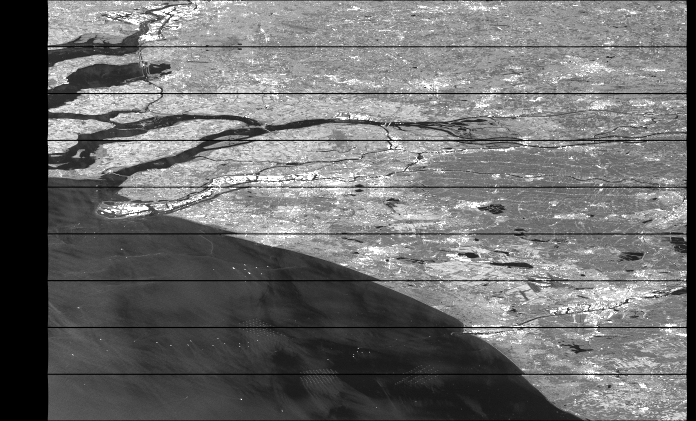
\includegraphics[width=0.5\linewidth]{f/slc_nvv_whole.png}
	&
	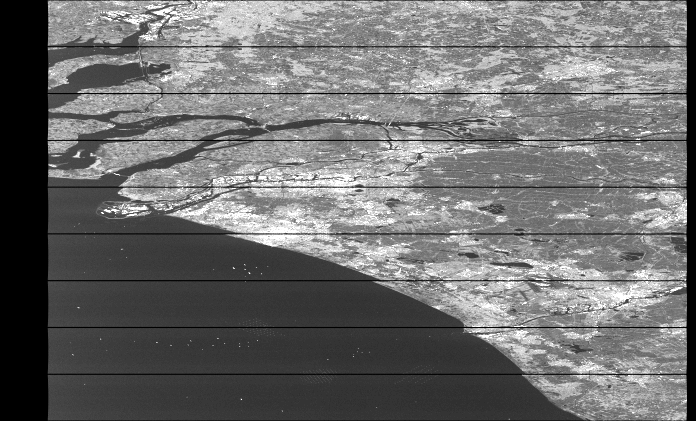
\includegraphics[width=0.5\linewidth]{f/slc_nvh_whole.png}
	\\
	norm(vv iw1) &
	norm(vh iw1)\\
\end{tabular}
\end{frame}

\begin{frame}\ttfamily
AN EXAMPLE RADAR IMAGE: FALSE COLOR\\
===================================\\
$ $\\

1 SLC datum = 6 complex images of size 20.000 x 15.000 \\
	{\color{gray} (vv, vh) x (iw1, iw2, iw3)}\\

	\vfill

	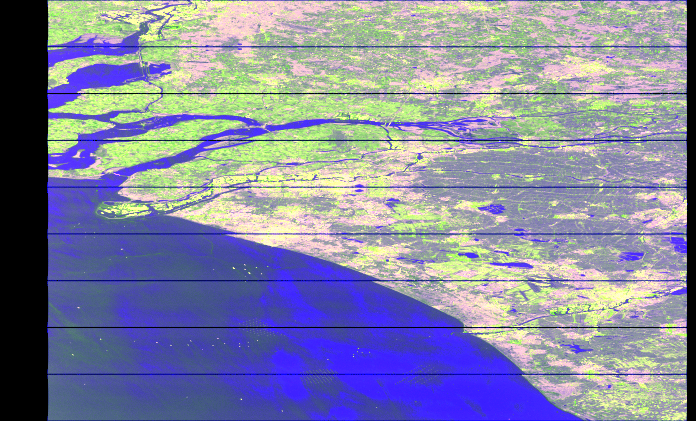
\includegraphics[width=0.8\linewidth]{f/slc_fc_whole.png}\\
	(R, G, B) = (|VH|, |VV|, $\alpha$ |VH|/|VV|)\\
	{\bf only iw1}
\end{frame}

\begin{frame}\ttfamily
AN EXAMPLE RADAR IMAGE: SWATHS\\
==============================\\
$ $\\

	1 SLC datum = 6 complex images of size 20.000 x 15.000 \\
	{\color{gray} (vv, vh) x (iw1, iw2, iw3)}\\

	\vfill

	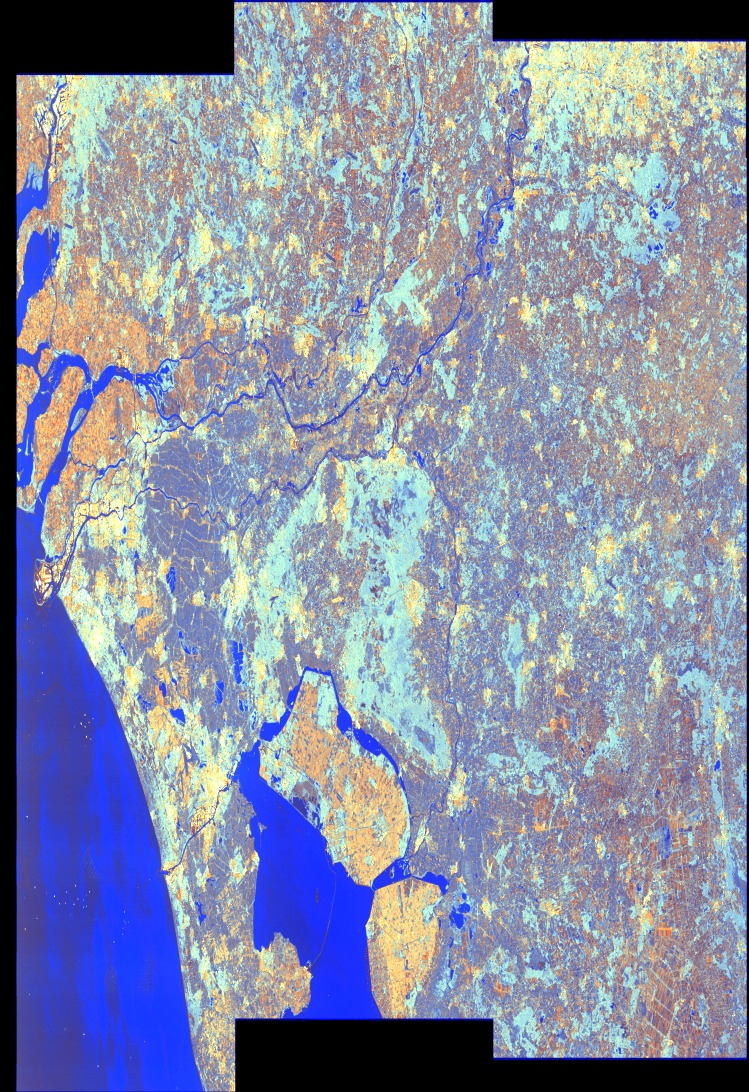
\includegraphics[width=0.4\linewidth]{f/rquick-look.jpg}
	$ $ merging of {\bf iw1, iw2, iw3}
\end{frame}

\begin{frame}\ttfamily
AN EXAMPLE RADAR IMAGE: DETAIL\\
==============================\\
$ $\\

	1 SLC datum = 6 complex images of size 20.000 x 15.000 \\
	{\color{gray} (vv, vh) x (iw1, iw2, iw3)}\\

	\vfill

\begin{tabular}{cc}
	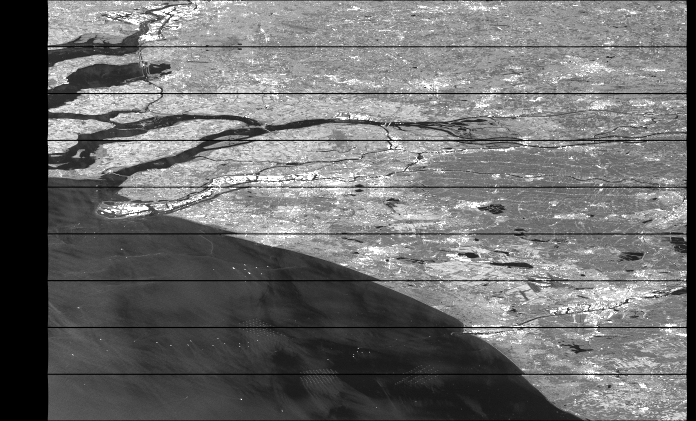
\includegraphics[width=0.5\linewidth]{f/slc_nvv_whole.png}
	&
	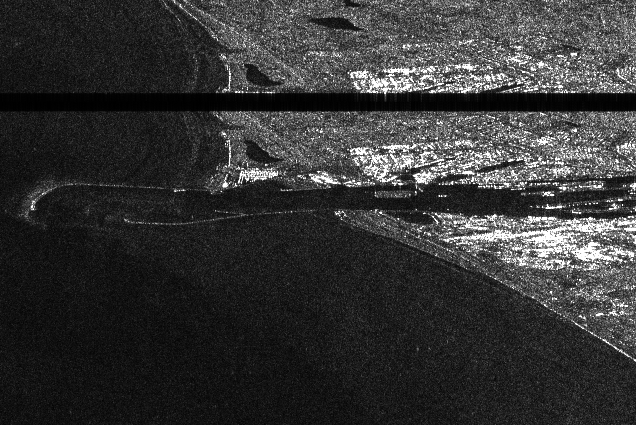
\includegraphics[width=0.5\linewidth]{f/slc_nvv_detail.png}
	\\
	|VV|, whole &
	|VV|, detail 1200x800 \\
\end{tabular}
\end{frame}

\begin{frame}\ttfamily
AN EXAMPLE RADAR IMAGE: COMPLEX NUMBERS\\
=======================================\\
$ $\\


\vfill
	(explore real/imag/angle, RAMPING)

	\vfill\color{darkgray}
	\tiny http://boucantrin.ovh.hw.ipol.im:7788/static/slc/i.html

	\tiny cpu /home/coco/pro/queiroz/phoqueouzygne/data/slc\_vv\_iw2.\%d.tif

	\tiny cpu /home/coco/pro/queiroz/phoqueouzygne/data/nslc\_vv\_iw1.\%d.tif
\end{frame}


\begin{frame}%\ttfamily
%THE BEST INTRODUCTION TO S.A.R. IMAGING\\
%=======================================\\
\vfill
	{\bf Synthetic Aperture Radar: Of Bats and Flying Pianos}\\
	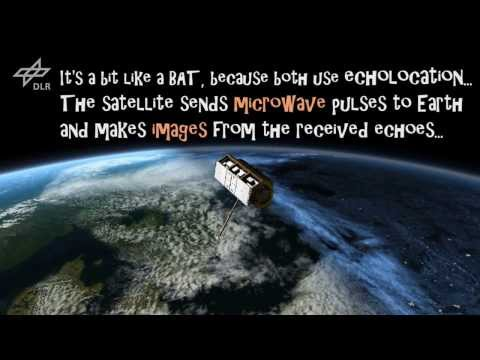
\includegraphics[width=0.9\linewidth]{f/bat.jpg}\\
	{\tt\color{blue} https://www.youtube.com/watch?v=g-YICKbcC-A}
\end{frame}

\begin{frame}\ttfamily
SAR IMAGING: HIGH-LEVEL VIEW\\
============================\\
$ $\\

	\begin{enumerate}
		\item The satellite emits a spherical signal~$f(t)$
		\item The objects in the ground reflect it
		\item The satellite receives the reflected signal~$g(t)$
		\item $I(x,y) = \mathrm{focusing}(g,x,y)$
	\end{enumerate}

	\vfill
	\pause
	\color{red}
	How to create a 2D signal $I(x,y)$ from a 1D signal~$g(t)$ ?
\end{frame}

\begin{frame}\ttfamily
AUDIO SPECTROGRAMS\\
==================\\
$ $\\

	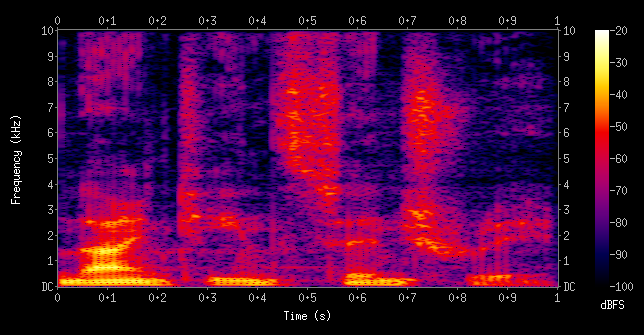
\includegraphics[width=\linewidth]{f/spectrogram.png}\\
	Spectrogram of the spoken words "nineteenth century"

\end{frame}

\begin{frame}\ttfamily
AUDIO SPECTROGRAMS\\
==================\\
$ $\\

	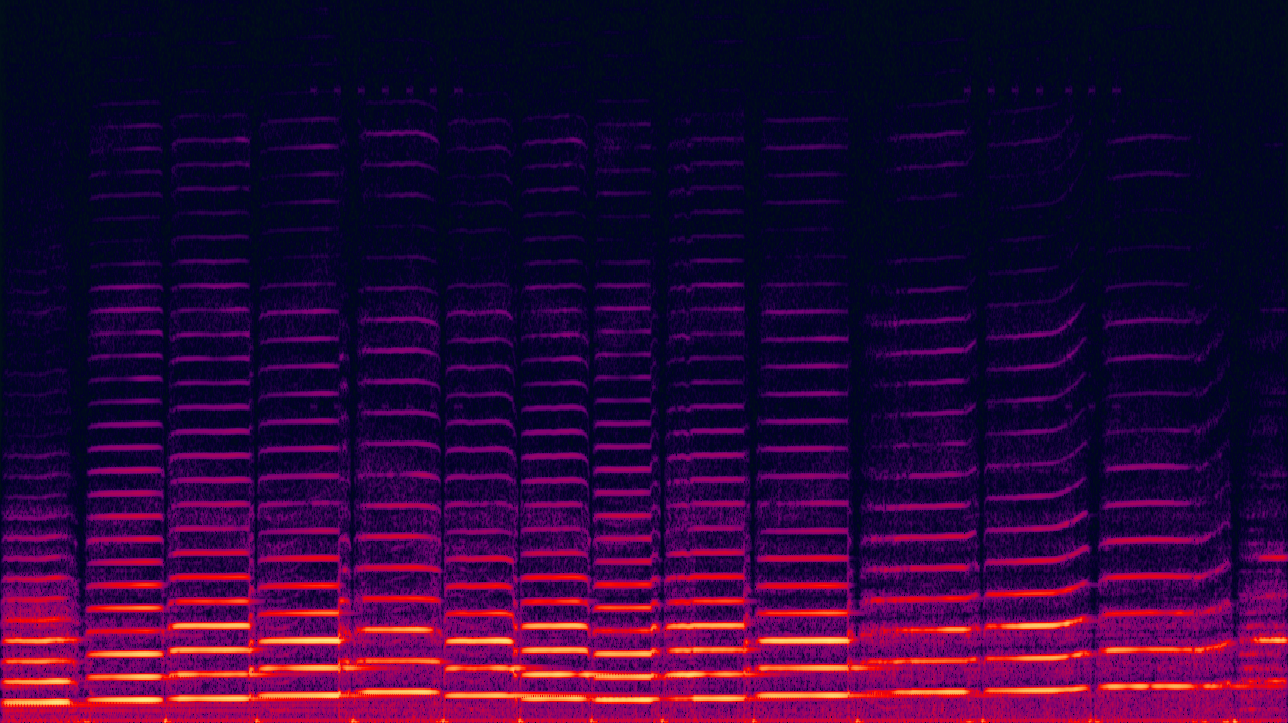
\includegraphics[width=\linewidth]{f/spec_violin.png}\\
	Spectrogram of a violin playing

\end{frame}


\begin{frame}\ttfamily
AUDIO SPECTROGRAMS\\
==================\\
$ $\\

	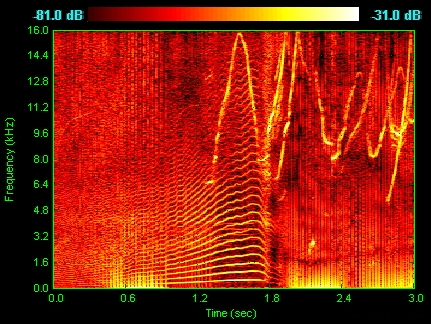
\includegraphics[width=0.7\linewidth]{f/spec_dolphin.jpg}\\
	Spectrogram of a dolphin

\end{frame}

\begin{frame}\ttfamily
GRAVITATIONAL SPECTROGRAMS\\
==========================\\
$ $\\

	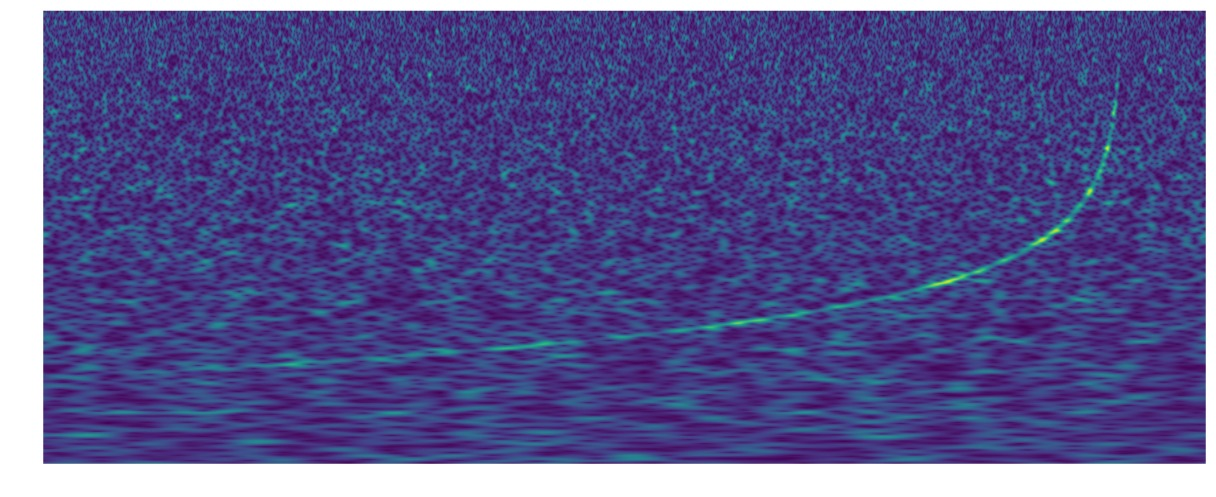
\includegraphics[width=\linewidth]{f/cspec_grav.jpg}\\
	Gravitational Wave {\bf GW170817}

\end{frame}

\begin{frame}\ttfamily
SPECTROGRAM STEGANOGRAPHY\\
=========================\\
$ $\\

	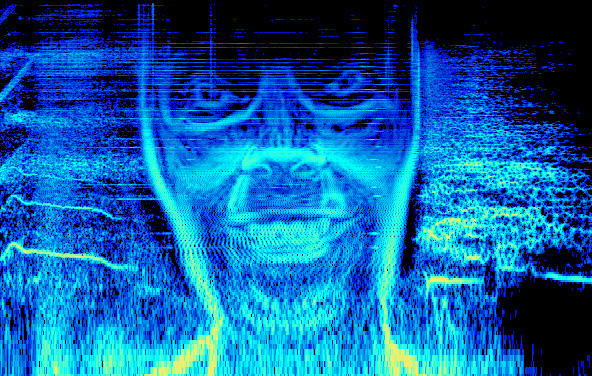
\includegraphics[width=\linewidth]{f/spec_steg.jpg}\\
	Fancy audio spectrogram (hand-edited)

\end{frame}

\begin{frame}\ttfamily
TIME-FREQUENCY ANALYSIS\\
=======================\\
\vfill

	\fbox{
	{\bf Input:} function $x(t)\qquad$ {\bf Output:} function $X(t,f)$
	}

	\vfill

Short-time Fourier transform (e.g., Gabor transform):
	\[
		X(t,f)=\int {\color{blue}w(t-\tau) e^{-if\tau}}x(\tau)\d\tau
		\qquad\qquad \mathrm{avec}\int w = 1
	\]

Wavelet transform:
	\[
		X(t,f)=\int {\color{blue}\frac{1}{\sqrt{f}}\varphi\left(\frac{t-\tau}{f}\right)}x(\tau)\d\tau
		\qquad\qquad \mathrm{avec}\int\varphi = 0
	\]

Wigner transform:
	\[
		X(t,f)=\int {\color{blue}e^{-if\tau}}
		x\left(t+\frac{\tau}{2}\right)
		\widebar{x}\left(t-\frac{\tau}{2}\right)
		\d\tau
	\]

\end{frame}

\begin{frame}\ttfamily
WHAT ARE SAR IMAGES\\
===================\\

\pause
\vfill
SAR images are spectrograms\\
\pause
\vfill


The analysis is performed using a {\color{blue}linear} chirp
	\[
		\color{blue}
		h(t) = \cos(t^2)
	\]
	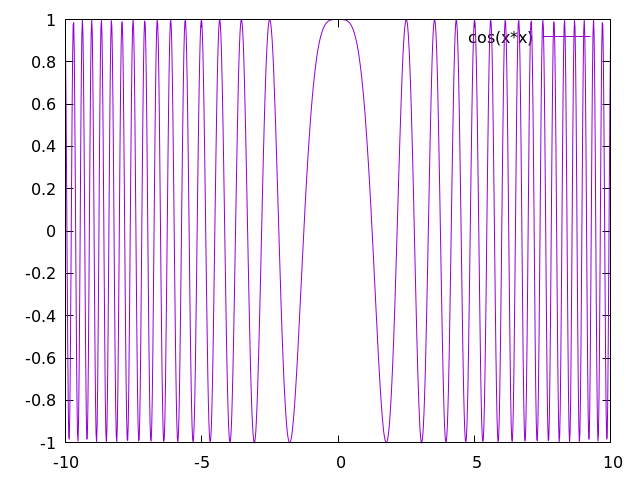
\includegraphics[width=0.6\linewidth]{f/costt.png}
\vfill
	{\scriptsize\color{red}Exercice: why is this function called a linear chirp?}
\end{frame}

\begin{frame}\ttfamily
THE MAGIC OF LINEAR CHIRPS\\
==========================\\
$ $\\

	Let~$h(t)=cos(t^2)$,  numerically, we will have $h\star h = \delta$.
	\vfill\pause

	More precisely, let~$h(t)=\mathrm{rect}\left(\frac{t}{T}\right)e^{iKt^2}$ and~$s_{out}=h\star h$.

	\vfill

	Exact formula:
	\[
		s_{out}(t)=(T-|t|)\mathrm{rect}\left(\frac{t}{2T}\right)
		\mathrm{sinc}\left(Kt(T-|t|)\right)
	\]

	\vfill

	Approximate formula (for $KT^2\ge 100$):
	\[
		s_{out}(t)=
		T\mathrm{sinc}\left(KTt\right)
	\]
\end{frame}

\begin{frame}\ttfamily
PRACTICAL CASE: SENTINEL 1\\
==========================\\
* Sentinel-1: ESA satellite that gives public images\\
* RAW : the received (quantized and encoded) raw data\\
* SLC : complex-valued images, obtained by focusing RAW\\
* GRD : complex-valued images, obtained by resampling SLC
\vfill
	\begin{tabular}{cccc}
		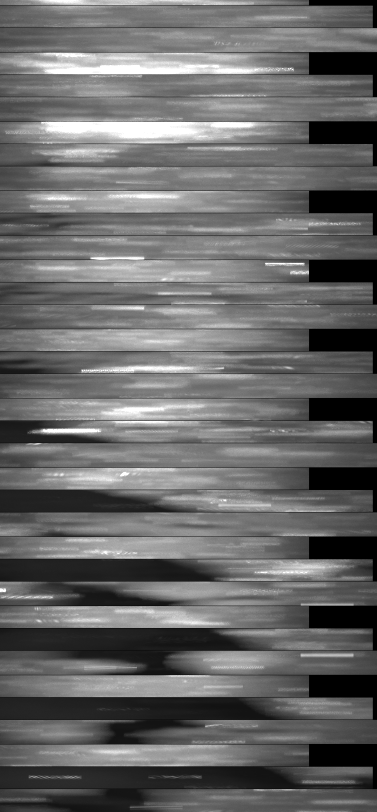
\includegraphics[width=0.23\linewidth]{f/xxx_norm6.png} &
		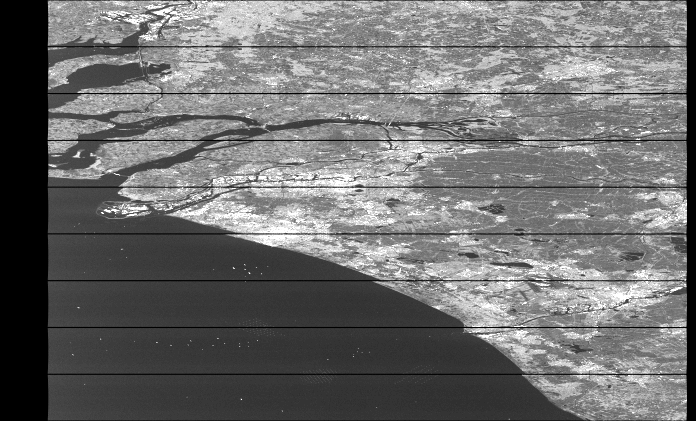
\includegraphics[width=0.23\linewidth]{f/vh5_iw1.png} &
		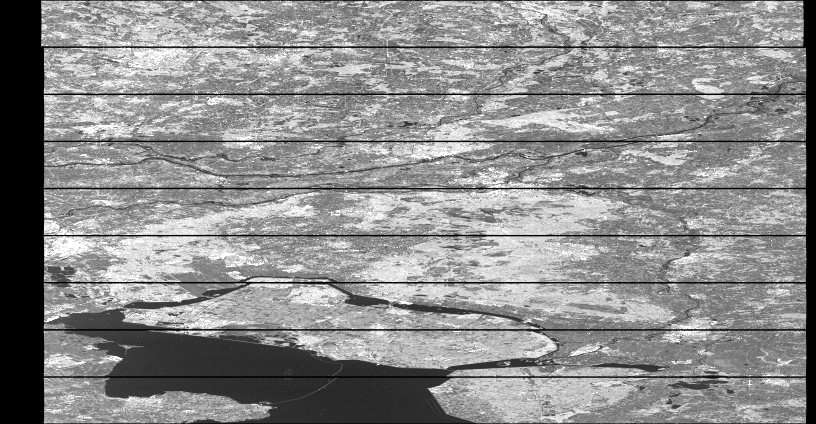
\includegraphics[width=0.23\linewidth]{f/vh5_iw2.png} &
		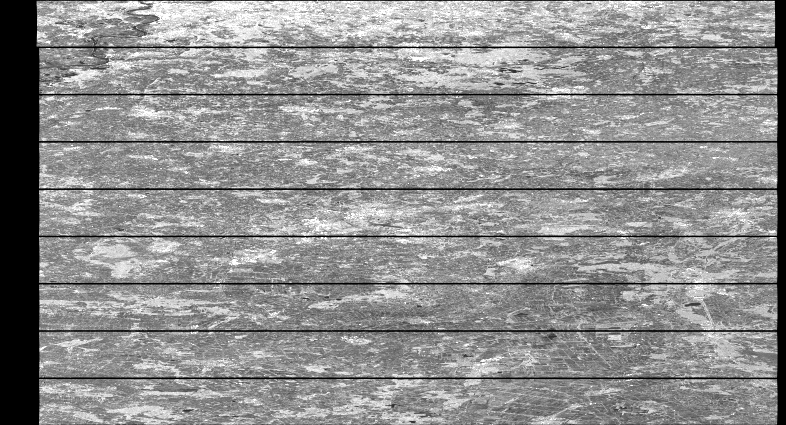
\includegraphics[width=0.23\linewidth]{f/vh5_iw3.png} \\
		\tiny RAW $24076\times51957$ &
		\tiny SLC${}_1$ $22288 \times 13473$ &
		\tiny SLC${}_2$ $26124 \times 13572$ &
		\tiny SLC${}_3$ $25173 \times 13617$ 
	\end{tabular}

\end{frame}

\begin{frame}\ttfamily
	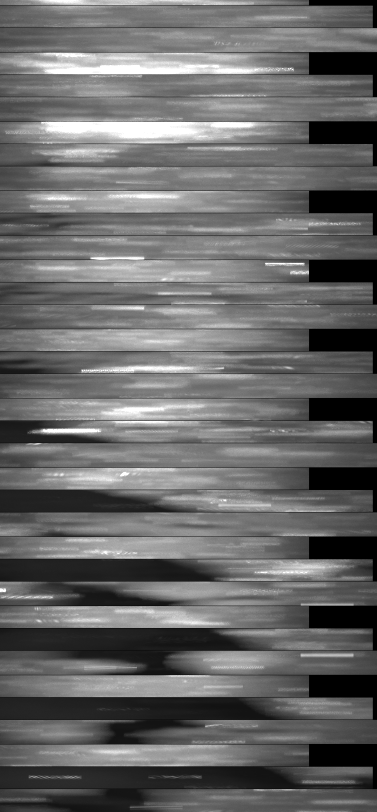
\includegraphics[height=0.99\textheight]{f/xxx_norm6.png}
	$ $
	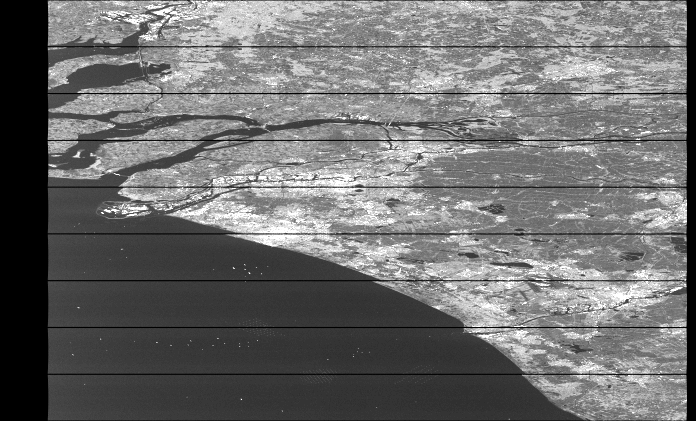
\includegraphics[height=0.4\textheight]{f/vh5_iw1.png}
\end{frame}


\begin{frame}\ttfamily
FOCUSING ALGORITHM\\
==================\\
$ $\\

{\bf Input:} Raw image~$R(x,y)$\\
{\bf Input:} Line range:~$y_a$, $y_b$\\
{\bf Output:} Focused part~$I(x,y)$\\

\begin{enumerate}
	\item Extract relevant lines $C(x,y)$ of~$R(x,y)$.
	\item $T$, $K$, $f$, $\ldots, \leftarrow$ parameters of $C(x,0)$.
	\item Correlate each line with~$h_{K_1,T_1}$
	\item Correlate each column with~$h_{K_2,T_2}$
	\item Output the resulting focused image~$I(x,y)$.
\end{enumerate}

\vfill
\pause
\color{red}
	{\bf Current state of affairs:}~$T_1$ and~$T_2$ are unknown, we estimate their best
values by visual inspection of the final result.

\end{frame}

\begin{frame}\ttfamily
VISUAL EXPLORATION OF FOCUSING PARAMETERS\\
=========================================\\
$ $\\

\vfill
	\color{gray}
	\tiny goto tmux clean ; fpanflip

\end{frame}

\begin{frame}\ttfamily
GOALS AND OPEN PROBLEMS\\
=======================\\
$ $\\

Why do we want to focus ourselves?\\
$\quad$* Intellectual curiosity\\
$\quad$* To focus images on a better-behaved grid\\
$\quad$* To adapt the focusing to a practical problem\\$\quad\ $ (e.g., detection of peaks)\\


\vfill
What is missing?\\
$\quad$* Find the exact parameters in the metadata\\
$\quad$* Understand the tradeoffs of different focusing algos\\
$\quad$* Implementation of the CLEAN algorithm

\vfill

\end{frame}

\end{document}



\end{document}


% vim:sw=2 ts=2 spell spelllang=en:
